\documentclass[review]{elsarticle}
\usepackage{graphicx}
\usepackage{amsmath}
\usepackage{enumerate}
\usepackage{multirow}
\usepackage{epstopdf}
\usepackage{array}
\usepackage{CJK}
\usepackage{float}
\usepackage{subfigure}
\usepackage{algorithm}
\usepackage{algorithmicx}
\newcommand{\algorithmicbreak}{\textbf{break}}
\newcommand{\BREAK}{\State \algorithmicbreak}
\usepackage{algpseudocode}
\newtheorem{problem}{\textbf{Problem}}
\usepackage{lineno,hyperref}
\modulolinenumbers[5]

\journal{Journal of \LaTeX\ Templates}

%%%%%%%%%%%%%%%%%%%%%%%
%% Elsevier bibliography styles
%%%%%%%%%%%%%%%%%%%%%%%
%% To change the style, put a % in front of the second line of the current style and
%% remove the % from the second line of the style you would like to use.
%%%%%%%%%%%%%%%%%%%%%%%

%% Numbered
%\bibliographystyle{model1-num-names}

%% Numbered without titles
%\bibliographystyle{model1a-num-names}

%% Harvard
%\bibliographystyle{model2-names.bst}\biboptions{authoryear}

%% Vancouver numbered
%\usepackage{numcompress}\bibliographystyle{model3-num-names}

%% Vancouver name/year
%\usepackage{numcompress}\bibliographystyle{model4-names}\biboptions{authoryear}

%% APA style
%\bibliographystyle{model5-names}\biboptions{authoryear}

%% AMA style
%\usepackage{numcompress}\bibliographystyle{model6-num-names}

%% `Elsevier LaTeX' style
\bibliographystyle{elsarticle-num}
%%%%%%%%%%%%%%%%%%%%%%%

\begin{document}

\begin{frontmatter}

\title{Exploiting Publication Contents and Collaboration Networks for Collaborator Recommendation}
%\tnotetext[mytitlenote]{Fully documented templates are available in the elsarticle package on \href{http://www.ctan.org/tex-archive/macros/latex/contrib/elsarticle}{CTAN}.}

%% Group authors per affiliation:
\author{Elsevier\fnref{myfootnote}}
\address{Radarweg 29, Amsterdam}
\fntext[myfootnote]{Since 1880.}

%% or include affiliations in footnotes:
\author[mymainaddress,mysecondaryaddress]{Elsevier Inc}
\ead[url]{www.elsevier.com}

\author[mysecondaryaddress]{Global Customer Service\corref{mycorrespondingauthor}}
\cortext[mycorrespondingauthor]{Corresponding author}
\ead{support@elsevier.com}

\address[mymainaddress]{1600 John F Kennedy Boulevard, Philadelphia}
\address[mysecondaryaddress]{360 Park Avenue South, New York}

\begin{abstract}
In academia, studies show that researchers are usually prolific by well collaboration with collaborators. However, due to the expansion of academic researches in diverse domains, the problem of finding most relevant and potential collaborators from a large volume of big scholarly data has become cumbersome and time-consuming. In this work, we propose an academic collaborators recommendation model called CCRec, an innovative model that combines content-based method with networks-based method. A topic clustering model and a random walk model are adopted to help effectively seek the most potential collaborators for researchers. Using DBLP data sets, we conduct benchmarking experiments to examine the performance of CCRec. Our preliminary experimental results show that CCRec outperforms other state-of-the-art methods in precision, recall and $F1$ score, additionally in addressing the topic drift problems.
\end{abstract}

\begin{keyword}
Collaboration recommendation, publication contents, collaboration networks, topic clustering, random walk.
\end{keyword}

\end{frontmatter}

\linenumbers


% =============================================================================
\section{Introduction}
% =============================================================================
Nowadays, with rapid development of Internet technology, the scale of Internet is beyond the imagination of people. Internet gradually becomes the main carrier of sharing information. Thus, how to obtain the useful one from vast information has become a complex task with the problem of information overload phenomena occurring. Therefore, recommender systems and techniques immensely help people by providing easier access to the specific resources they really need.

In academia, cooperation among researchers is of vital necessary. Studies show that researchers are usually prolific by well collaboration with collaborators \cite{lee2005impact}. This is to say, the collaborator is a considerable factor well connected with the productivity of a scholar. So researchers tend to discover the most potential collaborators (MPCs, some influential scholars who are similar in interests and have never collaborated with before), or reinforce the collaboration with the most valuable collaborators (MVCs, some influential scholars or colleagues who are active and valuable in adjacent circles and have ever collaborated). Considering the inherently requirements, there has been a variety of methods proposed recommending collaborators who they have ever collaborated with or never.

In this context, previous studies have exploited mainly three aspects for academic collaboration recommendation, content-based, social network-based and hybrid recommendation. [***references!***]Some traditional content-based methods represent researchers by interests tags, making collaborators recommendation by computing interests similarities.[***references!***] However, interests tags are sometime not accurately to represent researchers' features. Moreover, in general, a researcher shows bias on various academic domains. Such behaviors usually reveal academic features of researchers in different domains. Thus, it would be imperative considering academic domains when recommending collaborators. Our previous work proposed a networks-based model, ACRec \cite{li2014acrec}, which solved the problem of recommending MVCs. ACRec made it easier for scientists to collaborate with colleagues in their social networks. However, many scientists also initiate collaborations outside of their social networks. It is burdensome and fraught with risk of initiating collaboration with socially unconnected researchers. In addition, considering the less value of recommending already known collaborators, unconnected researchers are more deserve to be recommended as MPCs. What's more, some excellent hybrid models are offered in recent years \cite{lee2011recommending}, which provide us many good references.

In this paper, we propose a novel hybrid model exploiting publication contents and collaboration networks for collaborators recommendation (CCRec). Utilizing a topic clustering model \cite{pan2010research} \cite{pham2011clustering} and a random walk model, CCRec integrates the features of publications contents and collaboration networks. We extract the subject terms from all researchers' publications and cluster these terms into several topics, then distribute researchers to corresponding domains. To represent the feature vectors of each researcher, we run the random walk with restart model (RWR) on each domain, which has been proved to be competent for calculating the rank score of node in social networks. After that, the MPCs recommendation is provided by computing the similarities of researchers' feature vectors.

In summary, we make the following contributions in this paper. 1) To make the most potential collaborators recommendation, we develop a model CCRec, which combines the content-based method and social networks-based method. That is more favourable to achieve remarkable personalized collaborators recommendation. 2) To reveal researchers' academic features in different domains, we present the feature vectors by utilizing a topic clustering model and a random walk model. 3) We conduct extensive experiments on a subset of DBLP data set to evaluate the performance of CCRec in various scenarios as compared against our previous model ACRec and the normal common neighbors-based model (CNRec). Promising results are presented and analyzed.

The remainder of the paper is structured as follows. Section 2 briefly presents the related work. We discuss the details of our model in section 3, which highlights the structure of the model. In section 4, we conduct a mass of experiments and analyzes the results. At last, section 5 concludes the paper.

% =============================================================================
\section{RELATED WORK}
% =============================================================================
Collaboration plays an important role in academia research, a large body of works focuses on two key issues, reinforcing and discovering collaborators, which are respectively defined as MVCs recommendation and MPCs recommendation in this work. Lopes et al. \cite{lopes2010collaboration} work on identifying new partners to execute joint research and enhancing the cooperation of current partners for researchers. Chen et al. \cite{chen2009make} proposed that the purpose of friends recommendation is "Make new friends, but keep the old". Research on enterprise social networking \cite{dimicco2008motivations} shows that users in a corporate context are interested in discovering valuable contacts not yet known to them, or connecting to weak ties, in addition to staying in touch with their close colleagues. Our previous work \cite{li2014acrec} focus on recommending MVCs for researchers and enhancing the cooperation with colleagues in their academic social networks. In this work, CCRec have an aptitude for discovering new collaborators with high similarity (i.e. MPCs recommendation).

In general, collaborators recommender systems are studied in three different perspectives according to the methodologies used to perform recommendation: \emph{content-based}, \emph{social network-based} and \emph{hybrid approach}. The related works presented following are all correlation with these three types models.

\emph{content-based}, which recommends items classified accordingly to the user profile and early choices considering semantic issues. Das G. et al. \cite{gollapalli2012similar} propose models for computing the similarity between researchers based on expertise profiles extracted from their publications and academic homepages. Lopes et al. \cite{lopes2010collaboration} considered researchers' publications area and the vector space model to make collaboration recommendation. Kim et al. \cite{kim2010collaborative} propose a collaborative filtering method to provide an enhanced recommendation quality derived from user-created tags. However, researchers often behave differently across multiple domains of interests, therefore, there may be topic drift problems in general recommendation systems \cite{tang2012cross}.

\emph{social network-based}, which recommend items considering the structural of social network or some social factors. Ma et al. \cite{ma2011recommender} analysed how social networks information can benefit recommender systems and proposed a method improving the performance of recommender systems by incorporating social network information. T. Huynh et al. \cite{huynh2013trend} proposed a method based on combination of probability theory and graph theory for modeling and analysing co-author network. They explore the similar vertices as potential candidates for collaboration recommendation, their main contribution is taking the trend information into considering similarity of vertices. Many other approaches have been presented to formalize academic collaboration recommendation as a link prediction problem \cite{chen2012discovering} \cite{sun2011co} in social network. Some of these approaches have been applied to large social networks and results show a good performance. Lichtenwalter et al. \cite{lichtenwalter2010new} examined some important factors for link prediction and proposed a general framework, in addition to our previous work \cite{li2014acrec}.

\emph{hybrid}, which combines the content-based and social network-based to take advantage of their benefits. Lee et al. \cite{lee2011recommending} exploit how well content-based, social networks-based and hybrid recommendation algorithms predicted coauthor relationship, and the result show that a hybrid algorithm combining content and social networks information outperformed better. Chen et al. \cite{chen2011collabseer} discuss CollabSeer, an open system to recommend potential research collaborators for scholars and scientists, which discovers collaborators based on the structure of the coauthor networks and the user's topic of research interests. Cohen et al. \cite{cohen2013recommending} also work on solving the collaborators recommendation problem, by combining traditional techniques for structural link prediction in social networks with textual relevancy and global importance metrics.

% =============================================================================
\section{DESIGN OF CCRec}
% =============================================================================
Our proposed design scheme for CCRec is inspired by the reality and truth that a researcher usually desires to know other researchers who have similar research interests and strong influence in academia. As mentioned above, researchers often behave differently across multiple domains of interests. Such behaviors usually reveal academic features of researchers in different domains. Besides, as a social-based model, the RWR model has been proved to be competent for calculating the rank score of node in social networks derived from the co-authorship \cite{li2014acrec}, researchers' strength of influence in specific domains can be well reflected by RWR. In this work, we first adopt a content-based method to acquire multiple domains of interests. and then using the social network-based method of RWR to measure the researchers' strength of influence in different domains. After that, We use the feature vector to evaluate the similarity of researchers and then obtain the recommendation list. The detailed process is described bellow and the corresponding pseudo-code is illustrated in Algorithm 1. Figure 1 depicts three components of CCRec.

%Initially,

%In this work, we proposed a content-based method to acquire multiple domains of interests. Furthermore, we define the SoI (Strength of Influence) to denote the %academic values (Rank Score) of researchers in different domains, which can be regarded as the elements of feature vector of researchers. Finally,we use the %feature vector to evaluate the similarity of researchers and then obtain the recommendation list.
%Topic clustering and researcher partition distribute researchers according to multiple domains.
\begin{figure}
\centering
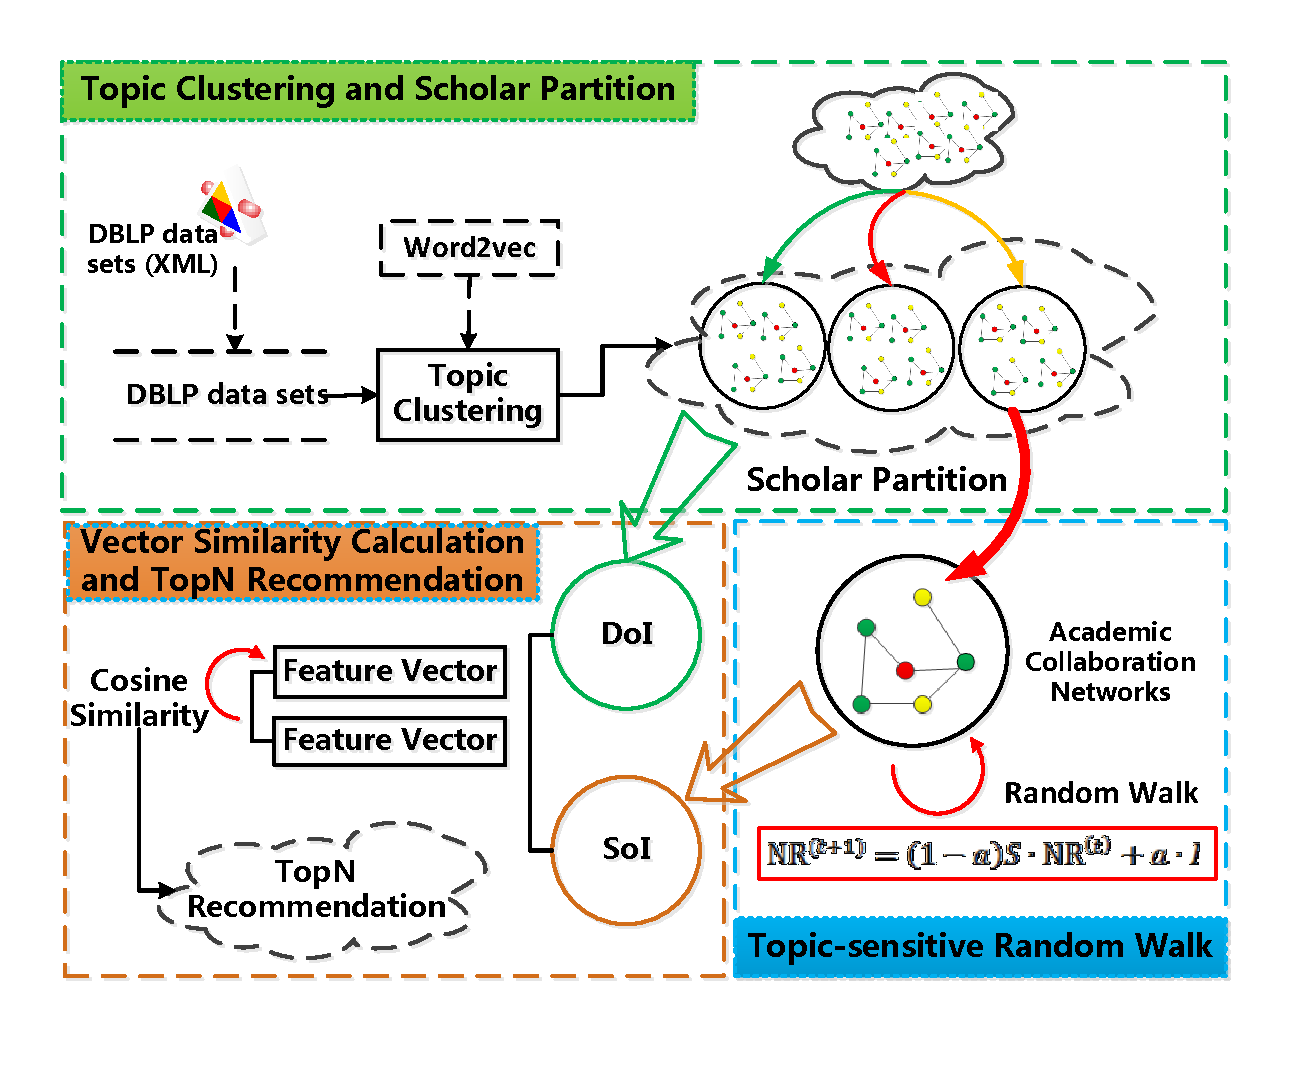
\includegraphics [width=4in]{Fig1.pdf}
\caption{The architecture diagram of CCRec model}
\end{figure}

\subsection{Topic Clustering and Researcher Partition}
% -----------------------------------------------------------------------------
It is a content-based method for topic clustering and researcher partition, which generates various domains and maps all researchers into these domains. In this work, we use a famous tool of NLP (Natural Language Processing), word2vec, which provides an efficient implementation of the continuous of \emph{bag-of-words} and \emph{skip-gram} architectures for computing vector representations of words. It takes a text corpus as the input and produces the word vectors as the output. The final word vector file can be used as features in many natural language processing and machine learning applications. The word vectors can be also used for deriving word classes from huge data sets. This is achieved by performing K-means clustering on top of the word vectors. The output is a vocabulary file with words and their corresponding domains IDs. In case of CCRec model, the input data is a set of titles from all the papers created by each researcher. The titles are split in many sequential words. In addition, there is necessary to filter out some irrelevant words, e.g. "of", "the", "and", etc. For extracting from titles, this set of preprocessed words can outline the core contents of papers, which are signified as valuable and reliable corpus to denote a variety of academic topics. With this English corpus, word2vec obtains various domains and clusters the words into the domains.

In addition, CCRec partitions researchers to specific domains with following method. 1, Extract subject terms from a researcher's publications. 2, Traverse all the terms and check the word vector. The model tags the researcher for particular domains which contains these subject terms. It should be emphasized that one researcher always belongs to several domains and there are also many researchers in one domain. Fig. 2 describe an example. Assuming that CCRec extracts 12 subject terms from the publications titles of researcher $S1$. After topic clustering, we can see that, three of these subject terms are assigned to domain $A$, and seven in $B$, two in $C$. Thus, researcher $S1$ is tagged for domains $A$, $B$ and $C$. Through this method, each domains contain numerous researchers.

\subsection{Feature Vector Calculation}
% -----------------------------------------------------------------------------
As mentioned in section 2, in general, researchers devote to several adjacent domains. But in the case of attention and strength of influence in various domains, they are offering some biases. To measure the distribution of researchers' interests, we define the $SoI$ (Strength of Influence) to denote the academic values (Rank Score) of researchers in different domains, which can be regarded as the elements of feature vector of researchers. Considering each of the domains, there are numerous researchers with similar research interests. Their co-author relationships can be modeled by a social network. Thus, there are many co-author networks corresponding to different domains. The $SoI$ is measured by RWR model based on the co-author networks. The core equation of the RWR model is shown below:
\begin{equation}
R_{d}^{(t+1)}=\alpha \mathbf{S}R_{d}^{(t)}+(1-\alpha)q
\end{equation}
where $R_{d}$ represents the rank score vector of all researchers in domain $d$, $q$ is the initial vector $R^0$, and $\alpha$ denotes the damping coefficient. RWR is an iterative process. After limited iterations, the vector $R$ will be convergent. In this scenario, $SoI_{s}=R_{d,s}$. That is, the final value of the vector item $R_{d,s}$ is the $SoI$ of researcher $s$.


In addition, with the help of RWR, The $SoI$ in various domains is quantified for each researcher. To measure researchers academic feature, we define the vector $F$ with $SoI$.

\begin{figure}
\centering
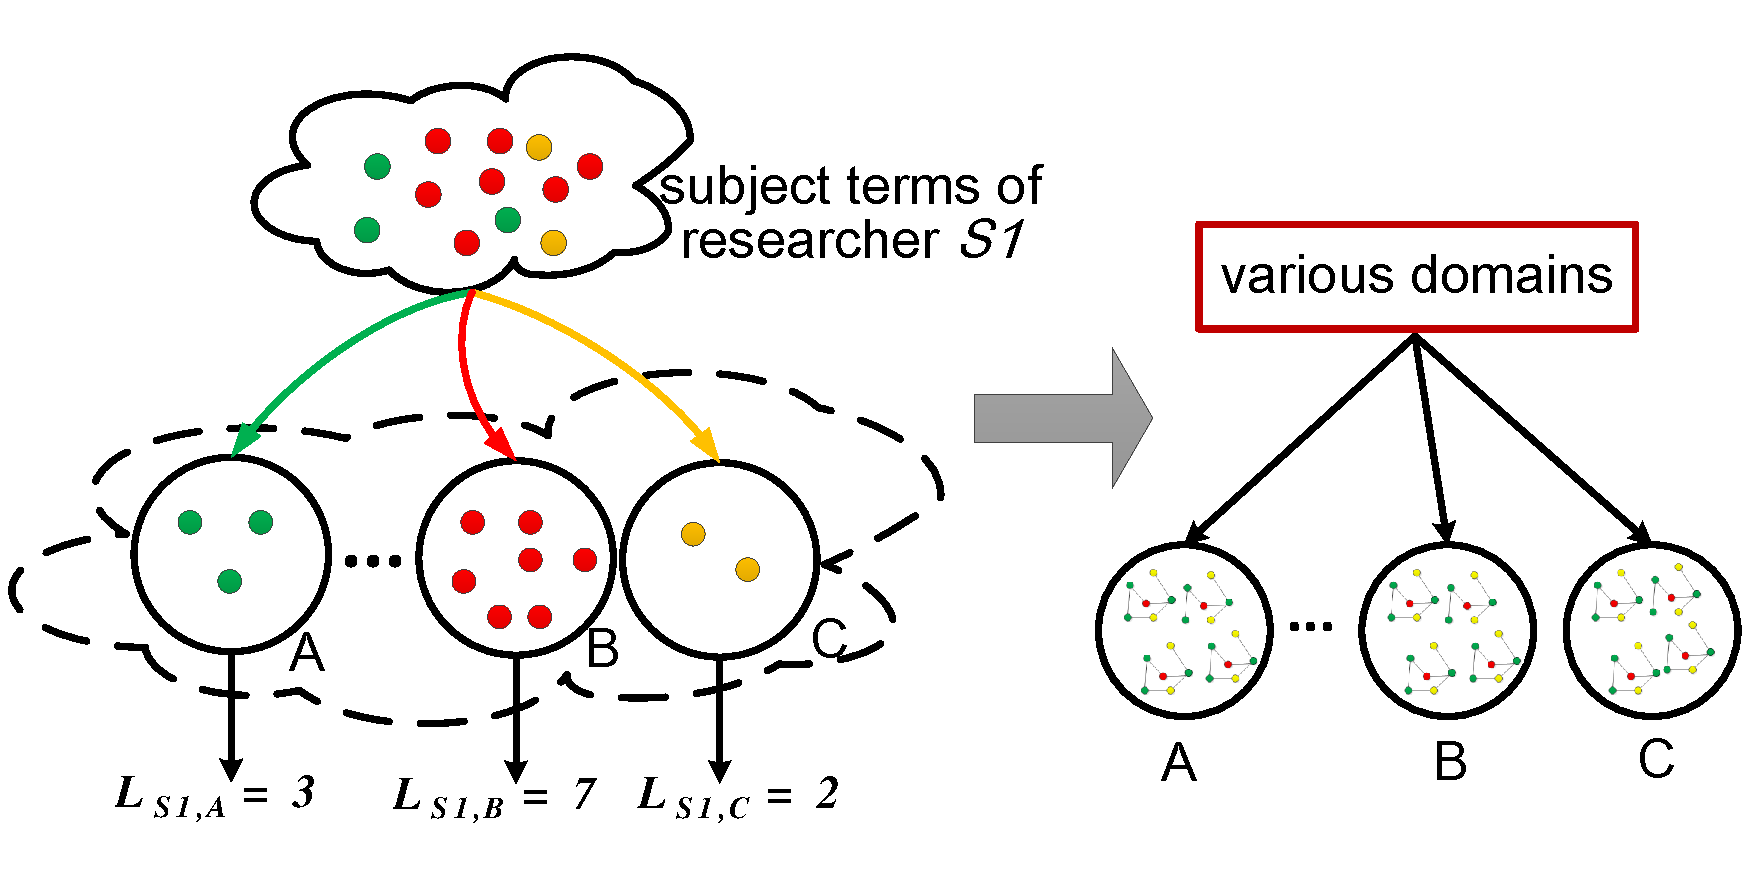
\includegraphics [width=4in]{Fig5.pdf}
\caption{Researcher Partition}
\end{figure}

\subsection{Collaboration Recommendation by Feature Vector Similarity}
% -----------------------------------------------------------------------------
CCRec recommends collaborators for researchers based on their similarities. To measure the academic features similarities of researchers, we borrow a standard method, \emph{cosine similarity} (CS). CS is employed to define the similarity between two users $s_{1}$ and $s_{2}$ based on their feature vectors $F_{s_{1}}$ and $F_{s_{2}}$.
\begin{equation}
Sim(s_{1},s_{2})=\frac{\sum_{i=1}^{n}(F_{s_{1},i}*F_{s_{2},i})}{\sqrt{\sum_{i=1}^{n}F_{s_{1},i}^2}*\sqrt{\sum_{i=1}^{n}F_{s_{2},i}^2}}
\end{equation}
Finally, we consider that researchers with high similarities have common interests, they should be recommended to each other as potential academic collaborators. Hence, CCRec provides a TopN recommendation list for each researcher.

% =============================================================================
\section{Evaluation and Analysis}
% =============================================================================
We conduct various experiments using data from DBLP \cite{Ley:DBLP}, a computer science bibliography website hosted at University Trier. We extracted the subsets of the entire data using the required information, which are all in the field of data mining involving 34 journals and 49 conferences. The data was modeled by an academic social network, which contains 59659 nodes (authors) and 90282 edges (coauthor relations). We divided the data set into two parts: the data before year 2011 as a training set, and others as a testing set.

We embarked on benchmarking experiments on CCRec. To evaluate the performance of CCRec model in a better way, we use three metrics which are widely used in the recommender systems, \emph{Precision}, \emph{Recall} and \emph{F1} \cite{shani2011evaluating}. We compared CCRec with the two following approaches. ACRec: a random walk recommendation model based on collaboration networks \cite{li2014acrec}. CNRec: a common neighbors based recommendation model \cite{lopes2010collaboration}. Four groups of experiments were conducted. 1, Find the most valuable collaborators, who may have known each other before, or be active in adjacent circles. 2, Recommend most potential collaborators, who have never cooperated with the target researcher before. 3, Evaluate how domains clustering impact the performance of CCRec. 4, Exploit the impact of clustered domains number on CCRec. For each experiment, we randomly chose 100 constant researchers who are at least somewhat active in academic activities, that is they have co-authored more than 30 person-time with others. We make collaborators recommendation for these 100 researchers, moreover compute the average of precision, recall and $F1$.

All experiments were performed on a 64-bit Linux-based operation system, Ubuntu 12.04 with a 4-duo and 32GHz Intel CPU, 4-G Bytes memory. All the programs were implemented with Python.

\subsection{Most Valuable Collaborators Recommendation}
% -----------------------------------------------------------------------------
In our previous work \cite{li2014acrec}, We proposed the ACRec model to make the most valuable collaborators recommendation for researchers. In this section, we explored the performance of CCRec and ACRec on making most valuable collaborators recommendation. The comparative results are shown in Fig. 2.

\begin{figure*}
\centering
\subfigure[Precision]{
\label{fig:2-a}
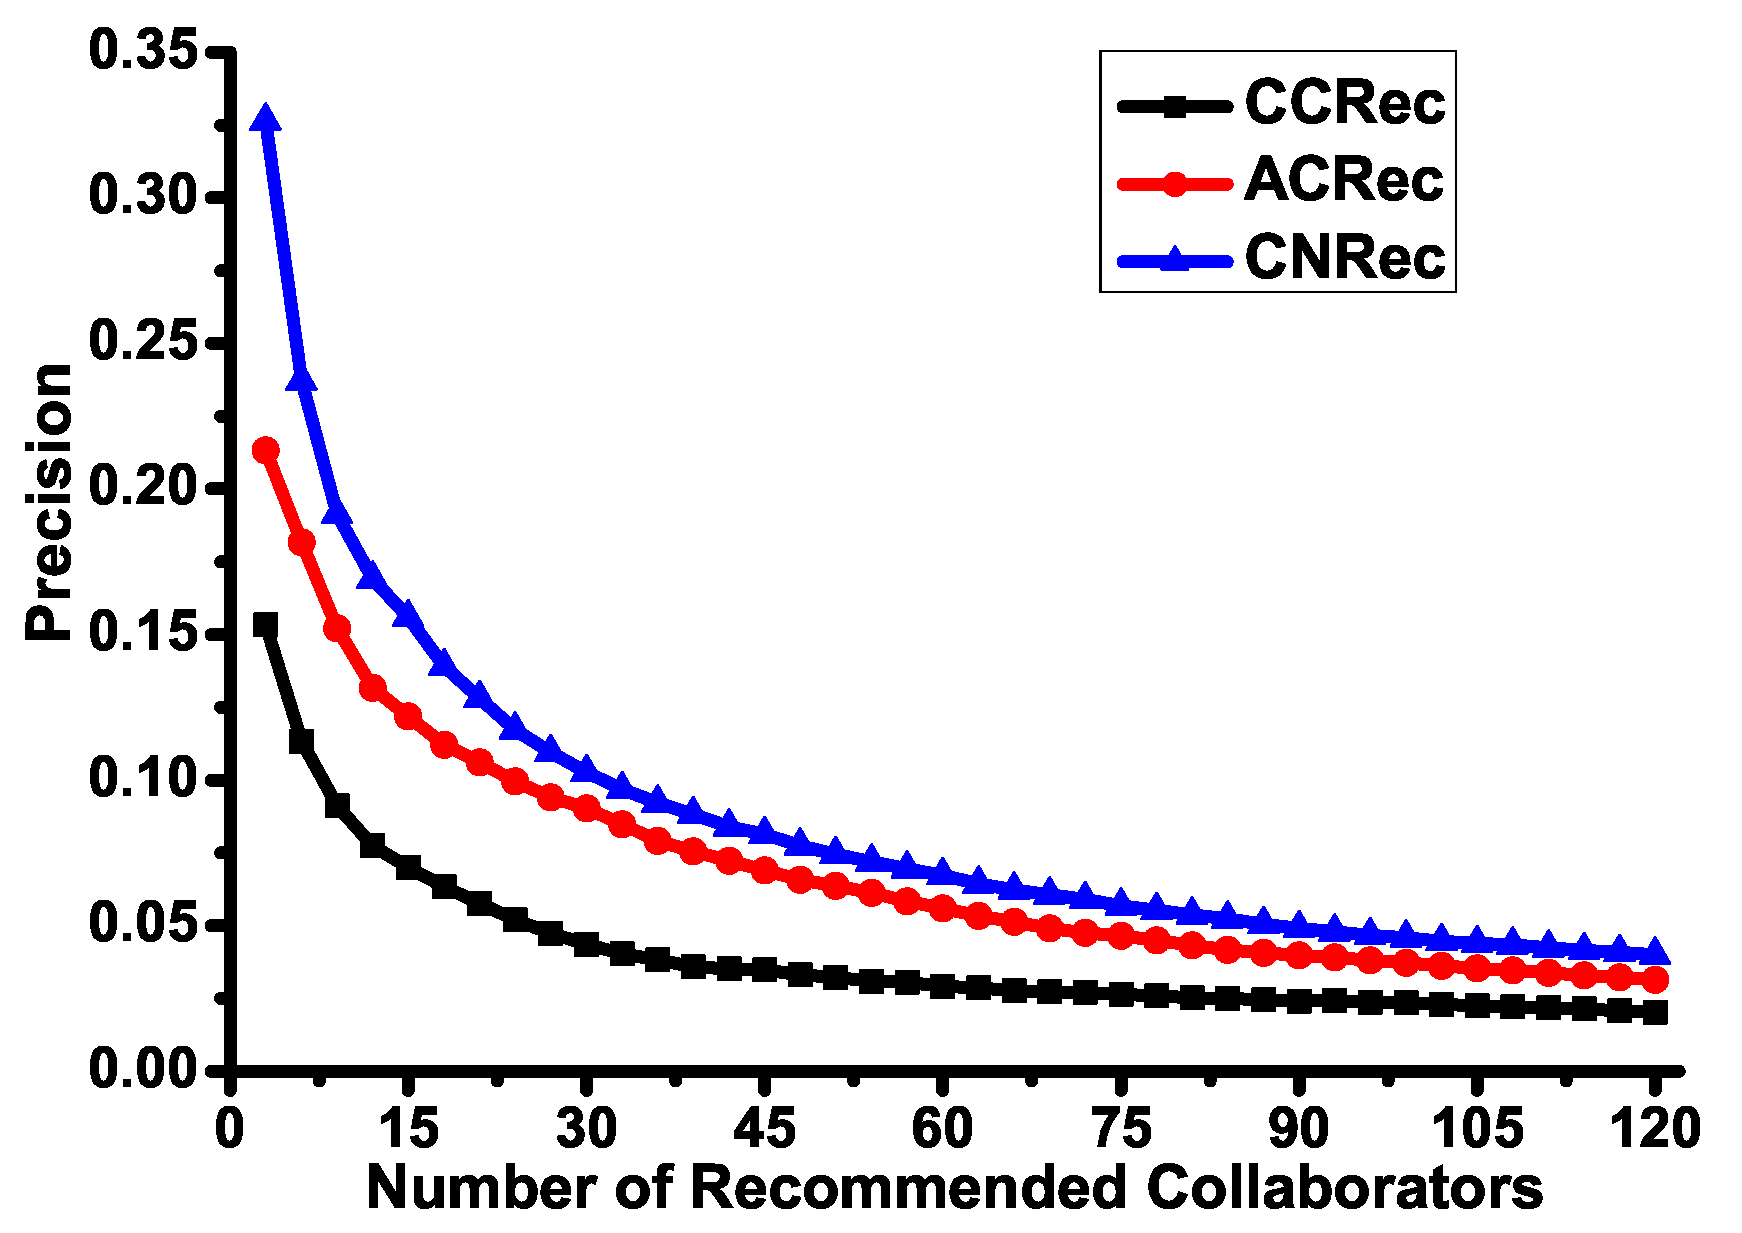
\includegraphics[width=0.31\textwidth]{Fig2-a.eps}}
\subfigure[Recall]{
\label{fig:2-b}
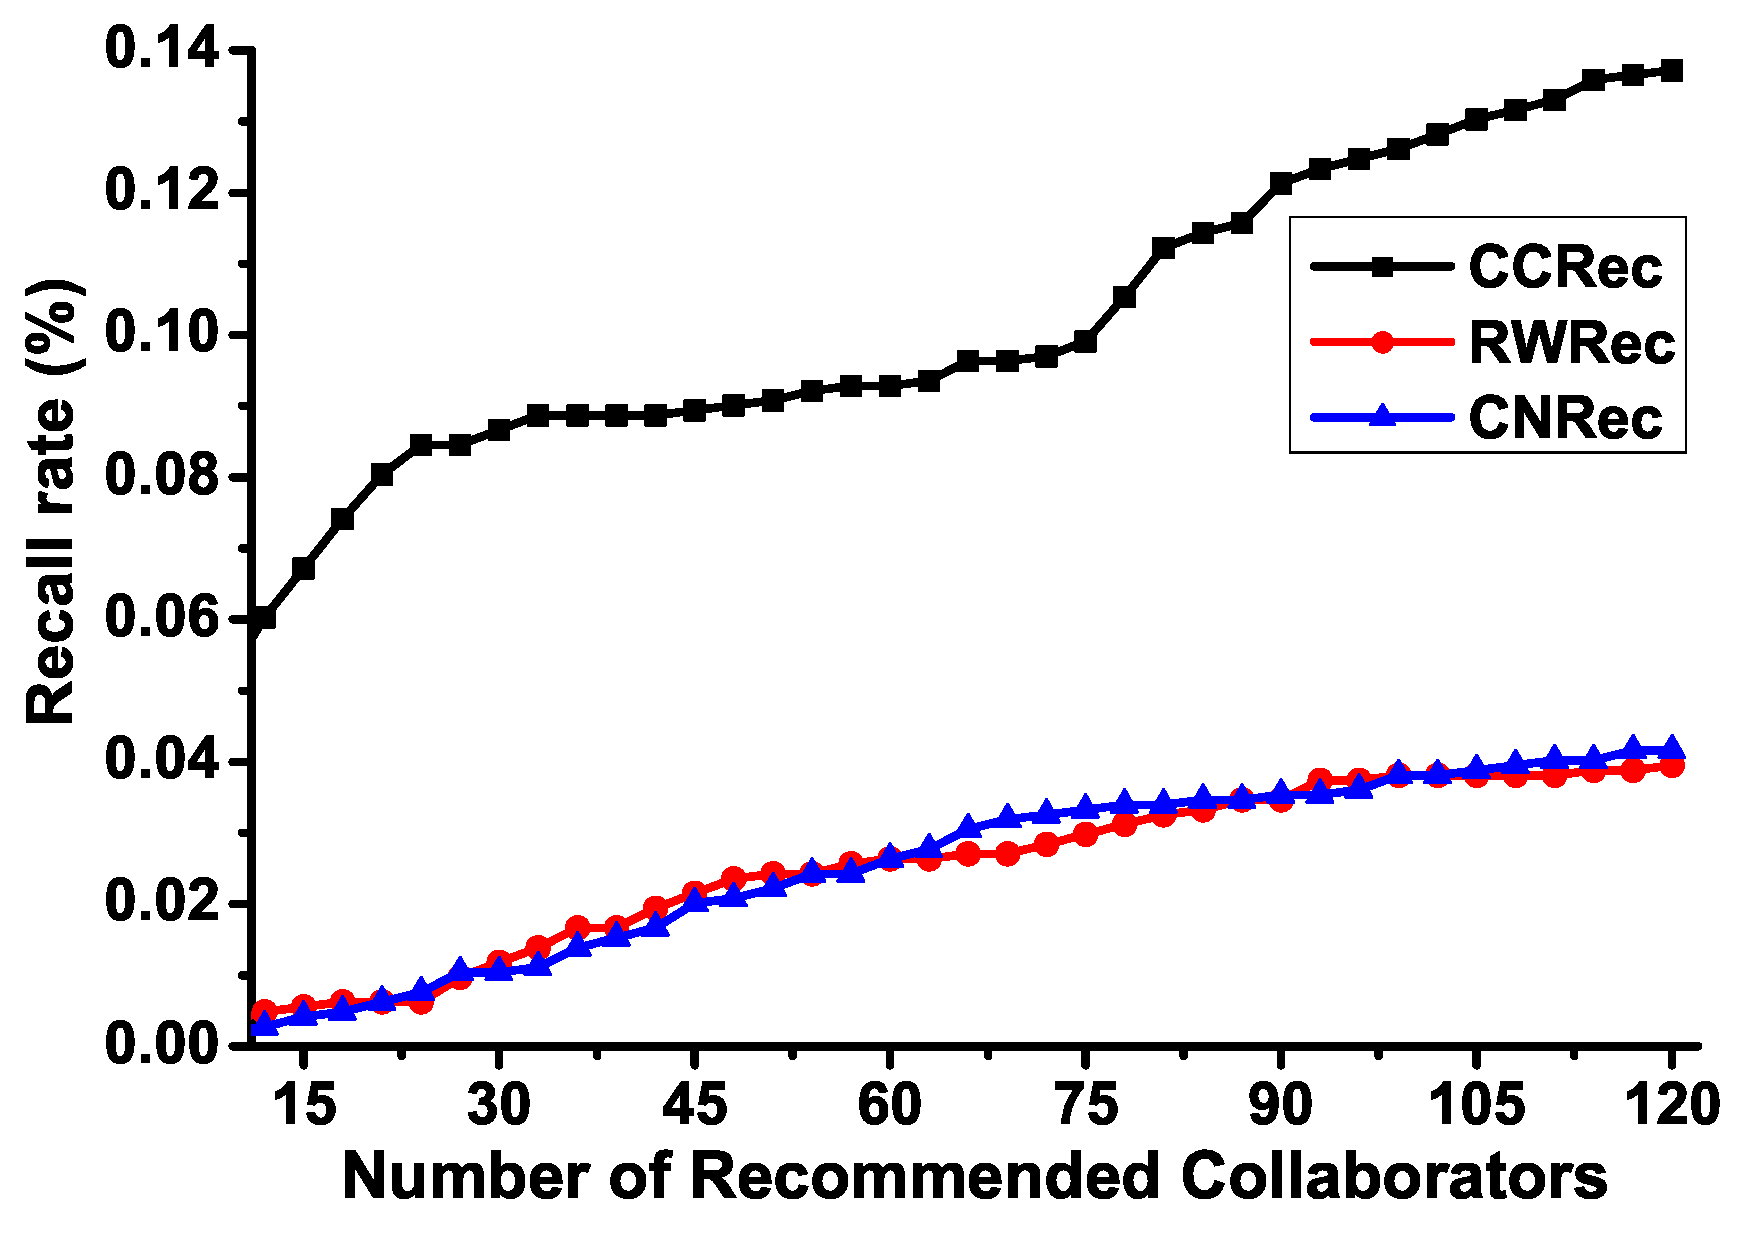
\includegraphics[width=0.31\textwidth]{Fig2-b.eps}}
\subfigure[F1]{
\label{fig:2-c}
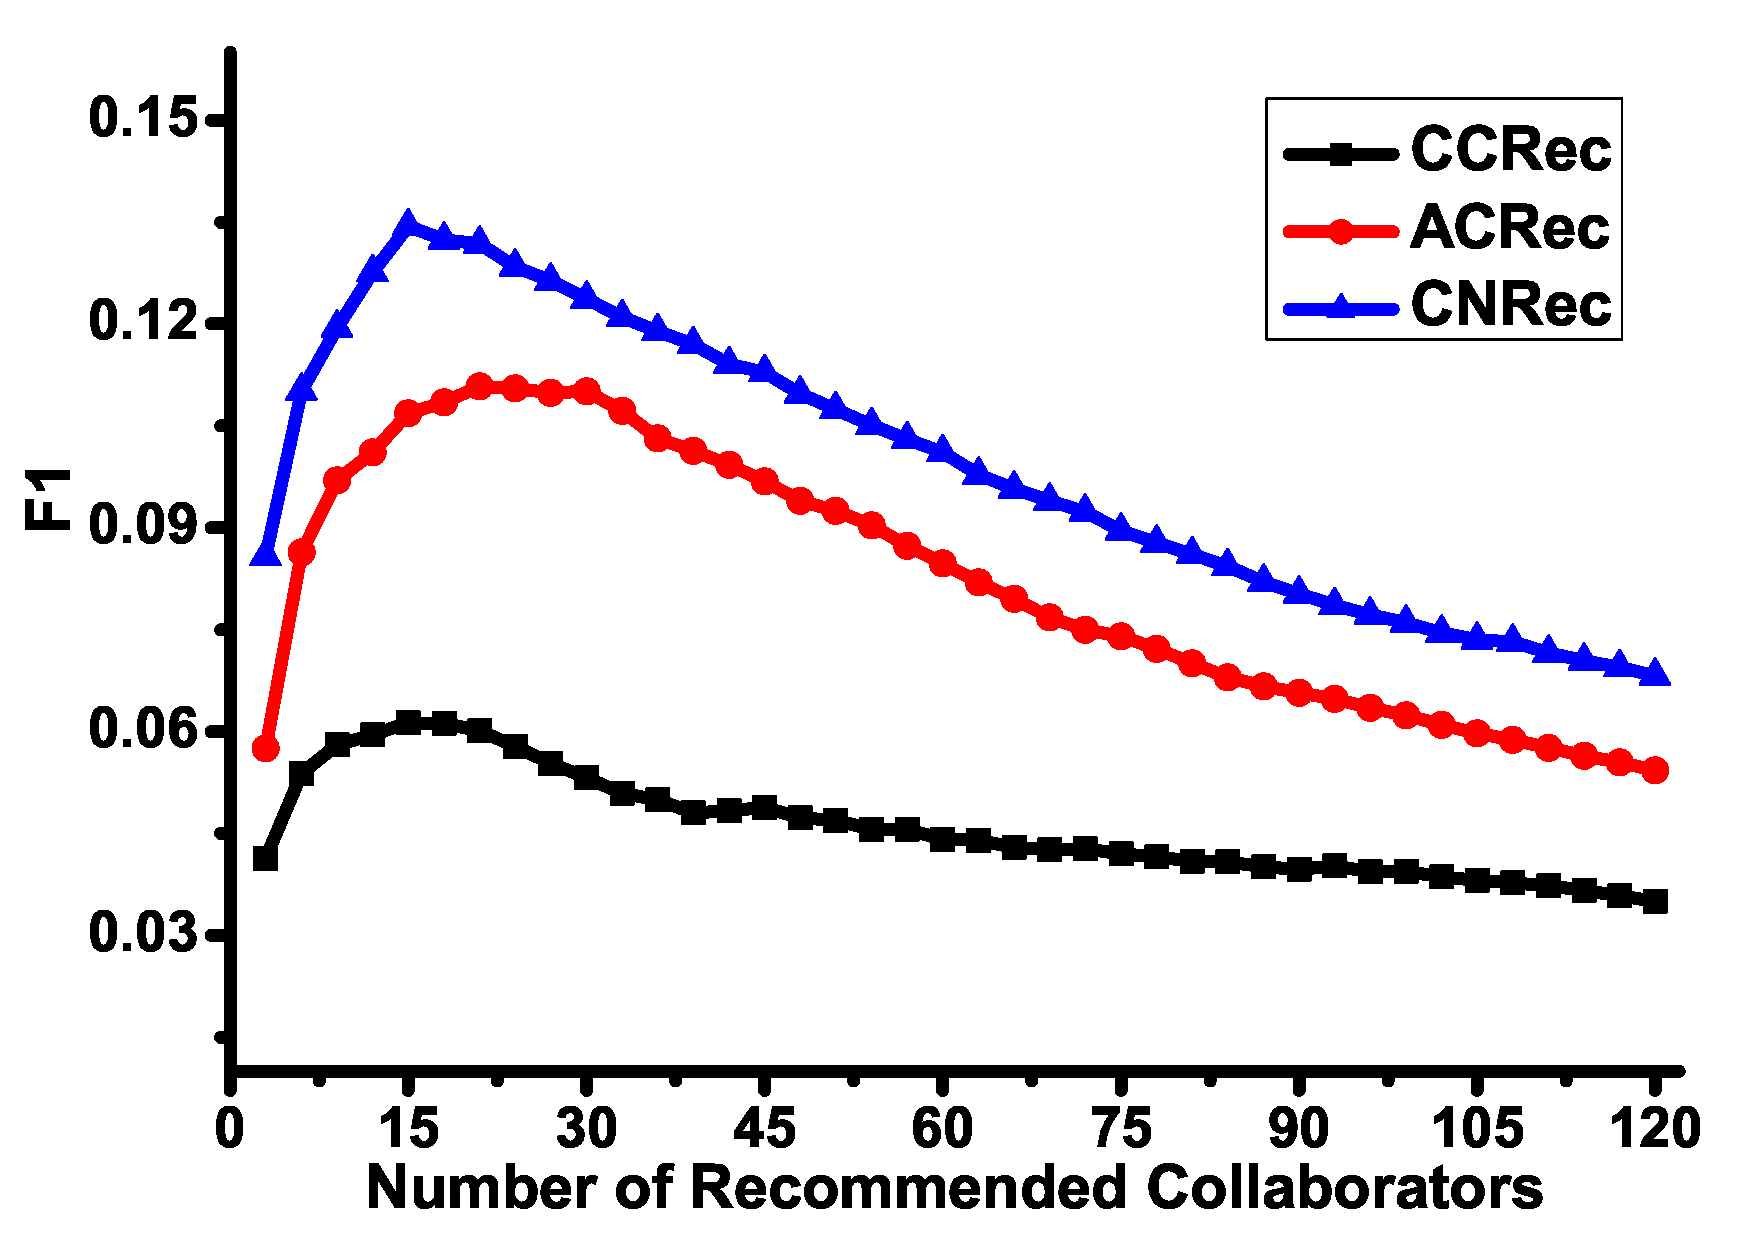
\includegraphics[width=0.31\textwidth]{Fig2-c.eps}}
\caption{Performance of CCRec and ACRec on most valuable collaborators recommendation}
\label{fig:2}
\end{figure*}

As shown in Fig. 2, The number of recommended collaborators has an obvious influence on the metrics with a clear trend. In the case of CCRec, as shown in Fig. 2(a), the precision drops when the number of recommended collaborators is increasing. At the same time, the recall in Fig. 2(b) rises with the increase of recommendation list, which approximates to $20\%$ in the end. As for ACRec, it has the same trend with CCRec on precision and recall. Thus it can be seen, the precision and recall are a pair of contradictory metrics. Weighing the two metrics to maximum the profit, G. Shani et al. \cite{shani2011evaluating} adopt the metric $F1$. Fig. 2(c) describes the performance of CCRec and ACRec on $F1$. In case of CCRec model, the $F1$ generally increases until the number of recommended collaborators is over 15, and then decreases gradually. Since the point 15 is exactly the peak of $F1$. We can see that, CCRec performs best when recommend 15 collaborators to each researcher, and the $F1$ can reach $6.13\%$. However, in this scenario, ACRec gets its' highest $F1$ score $11.01\%$ at point 30.

In terms of Fig. 2, It is  much in evidence that ACRec model outperforms CCRec model on making most valuable collaborators recommendation. This is because, ACRec based on the link-importance guiding random walk, considering the walk distance and rank score, seeks the most valuable collaborators who may have known each other before, or active in adjacent circles. Thus, compared with ACRec, there is no obvious superiority for CCRec to find the most valuable collaborators in adjacent circles.

\subsection{Most Potential Collaborators Recommendation}
% -----------------------------------------------------------------------------
We define the Most Potential Collaborators as collaborators who are worthy of being recommended and have never cooperated with the target researcher. Making the most potential collaborators recommendation is of great significance as the new collaborators are more meaningful and practical in academia reality. In this section, we explored the performance of CCRec, ACRec and CCRec on making most valuable collaborators recommendation.

\begin{figure*}
\centering
\subfigure[Precision]{
\label{fig:3-a}
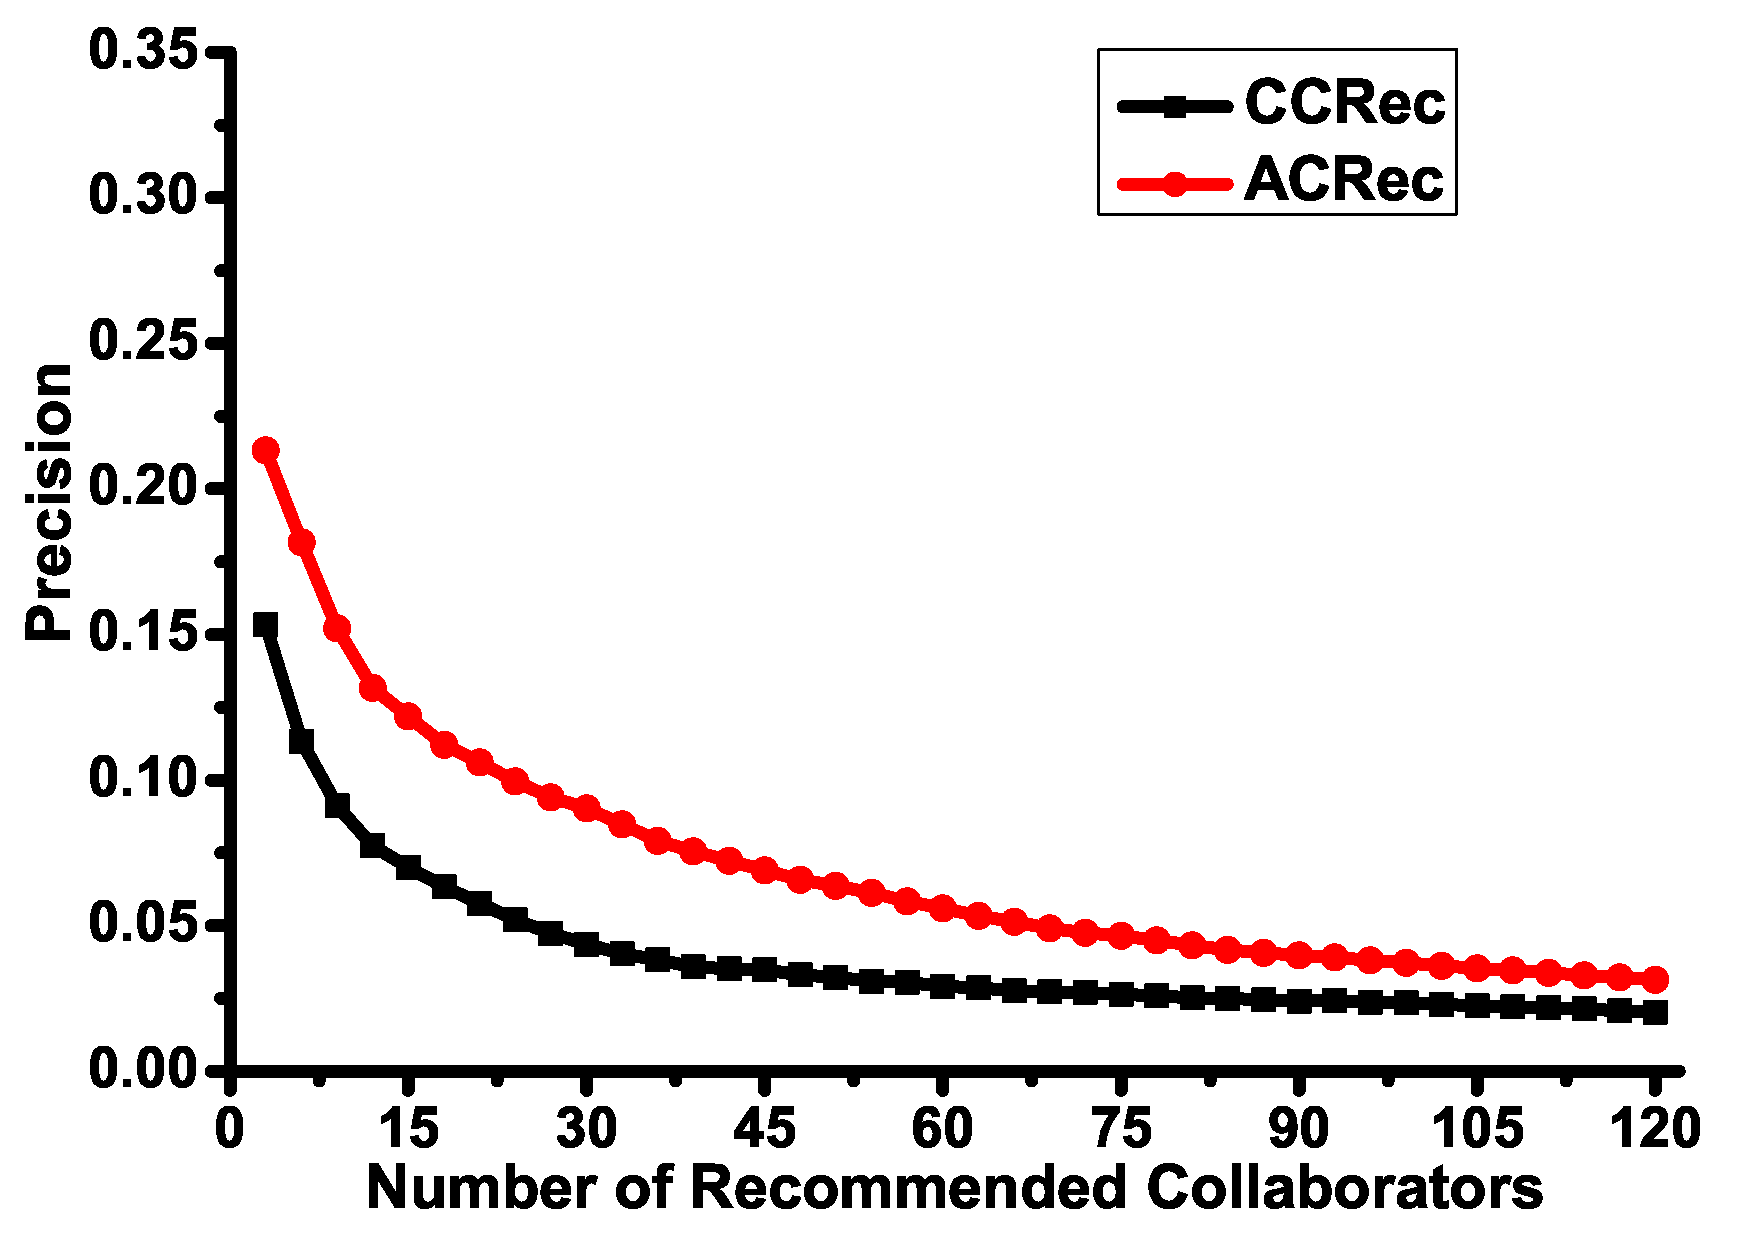
\includegraphics[width=0.31\textwidth]{Fig3-a.eps}}
\subfigure[Recall]{
\label{fig:3-b}
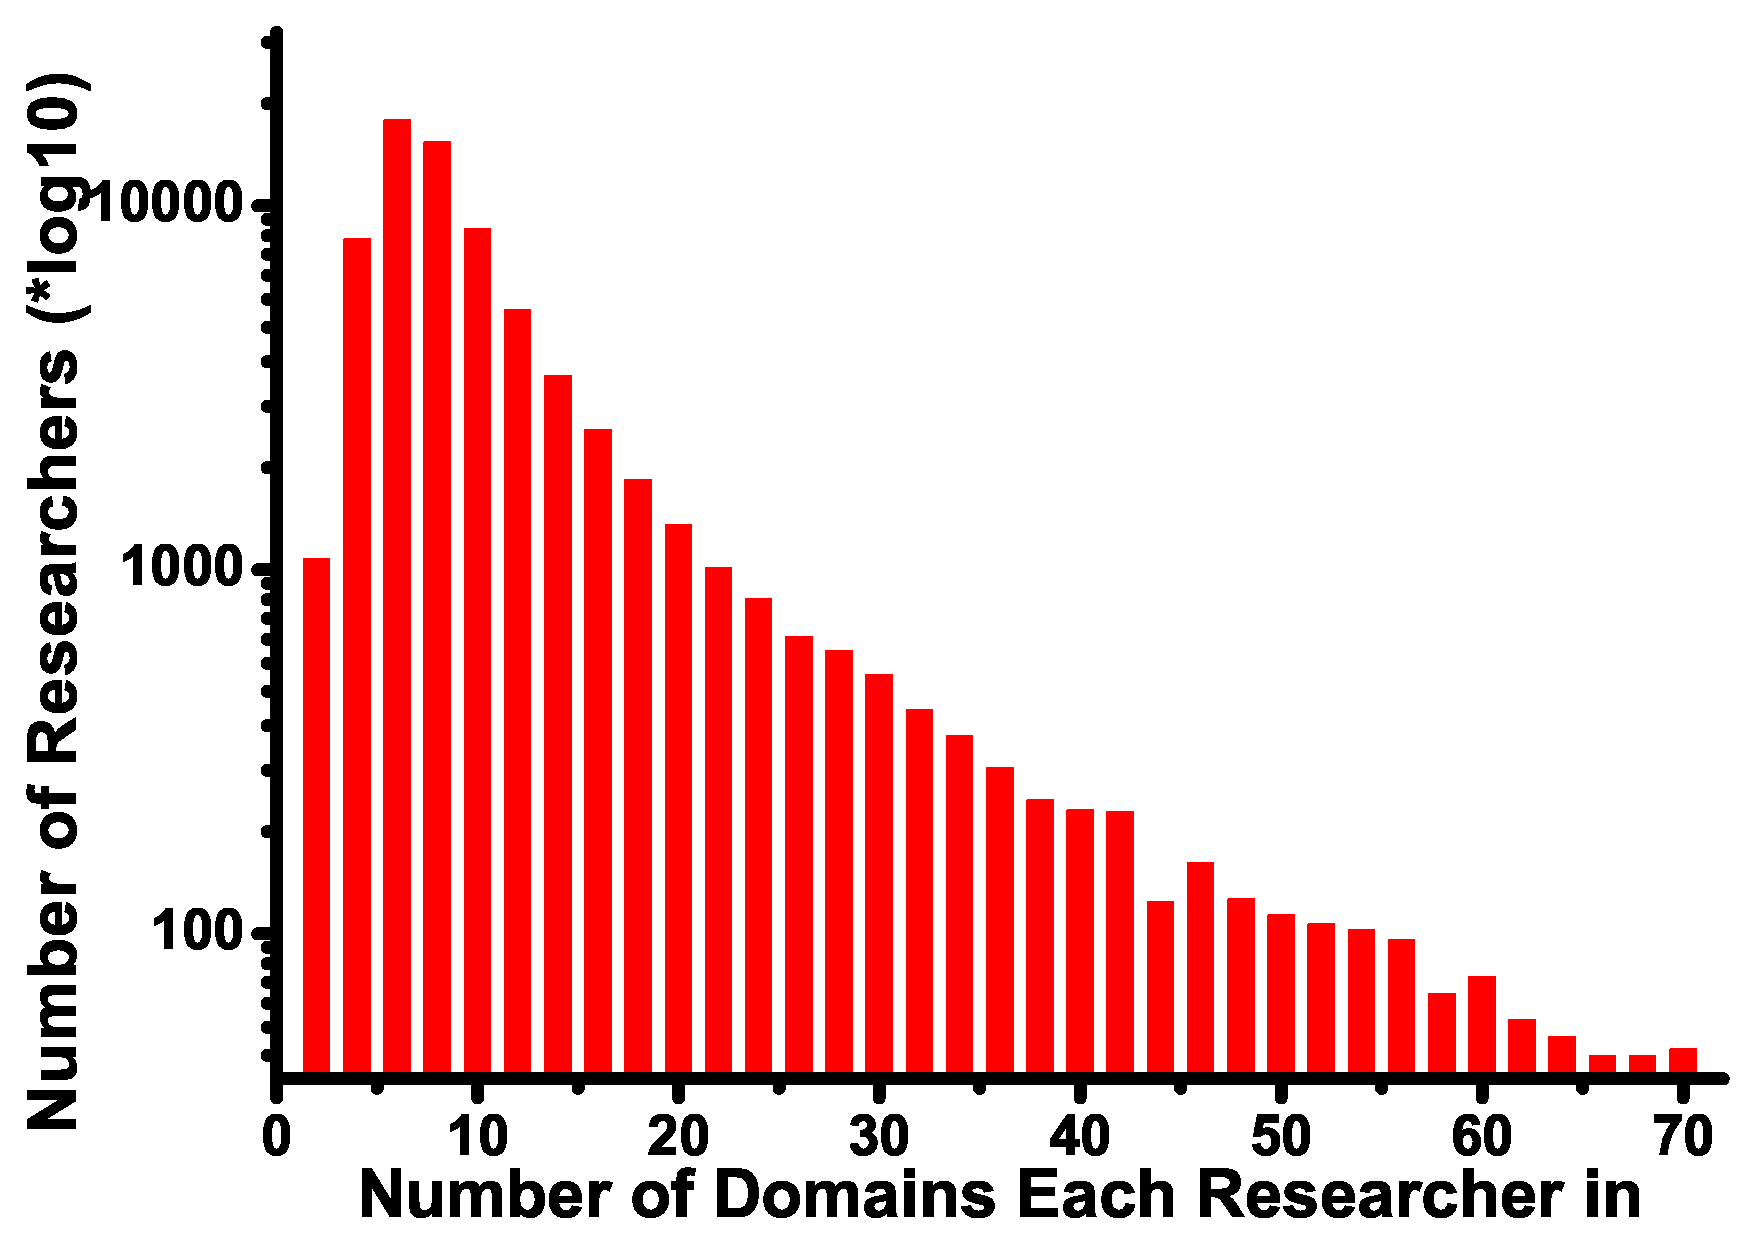
\includegraphics[width=0.31\textwidth]{Fig3-b.eps}}
\subfigure[F1]{
\label{fig:3-c}
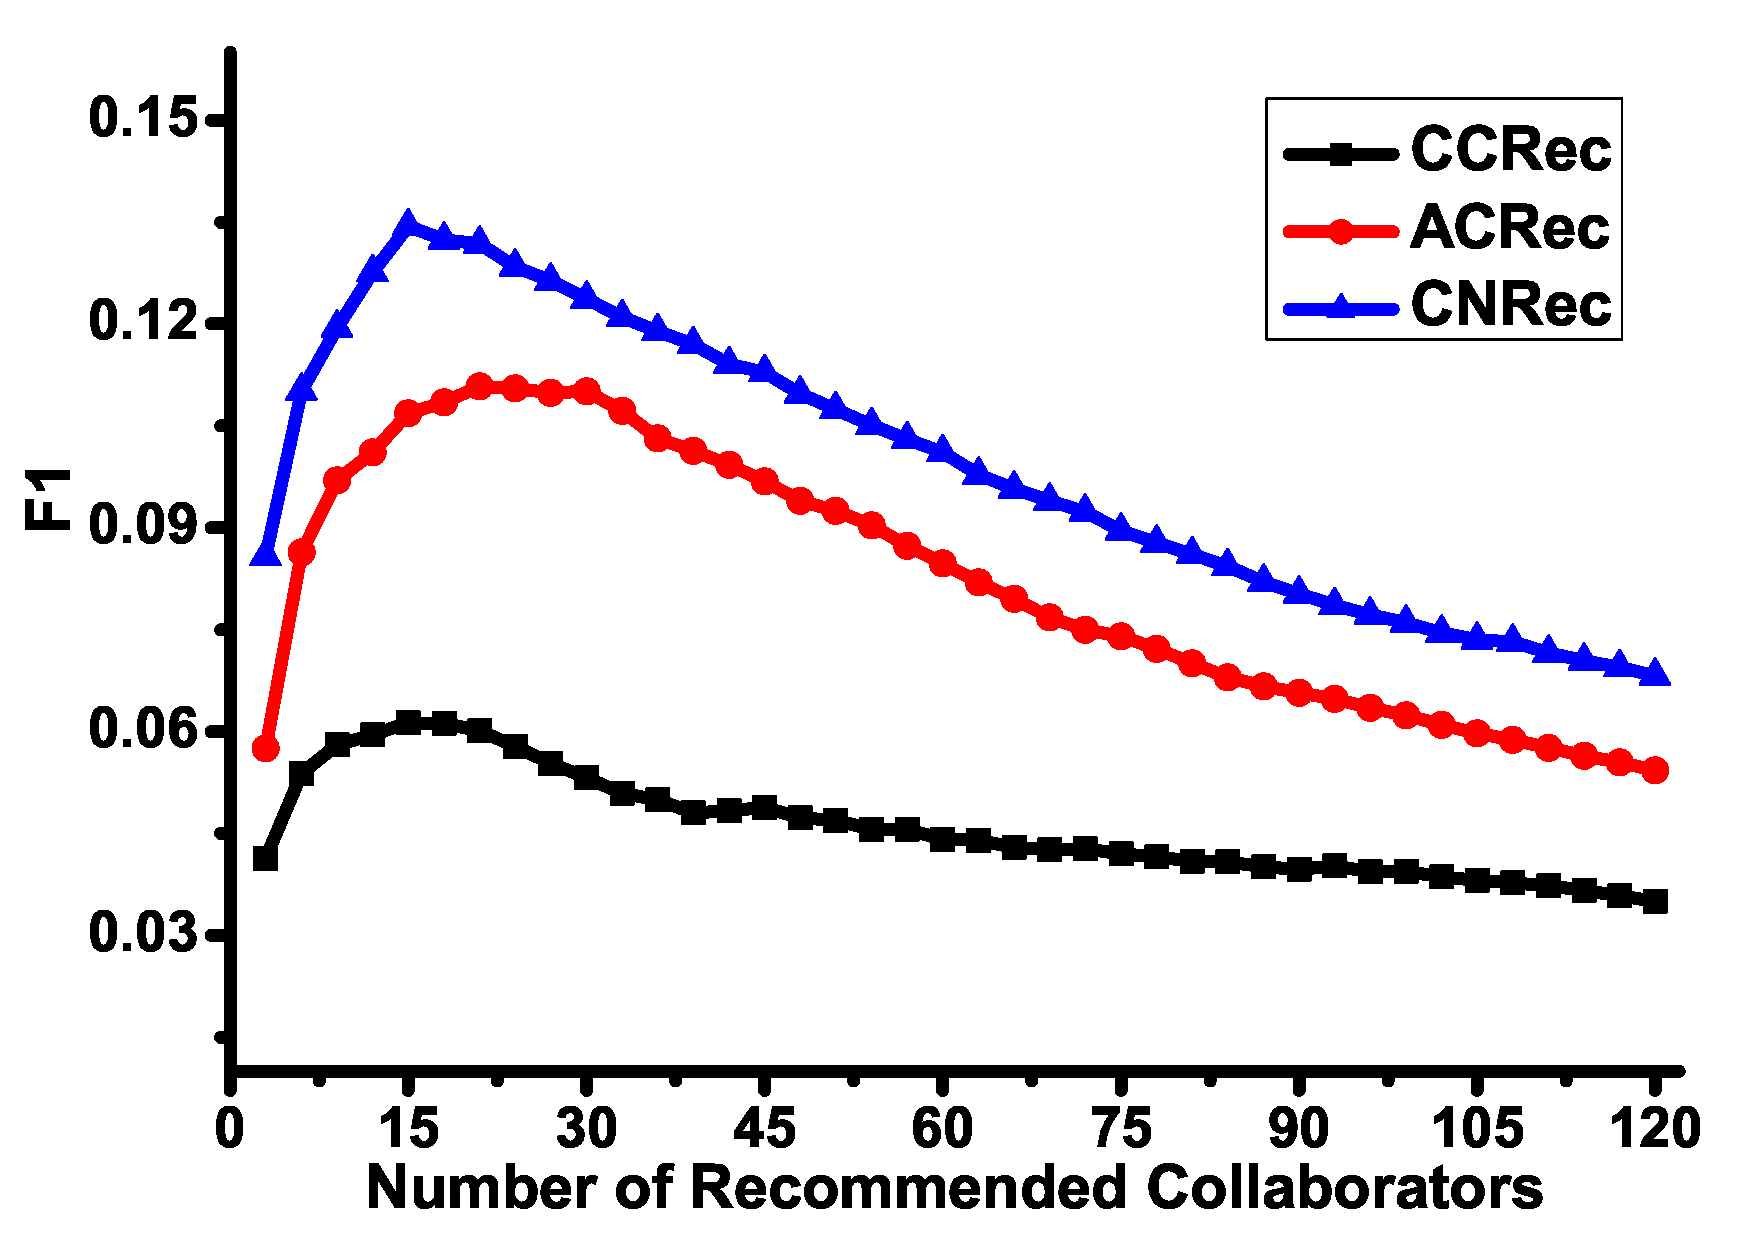
\includegraphics[width=0.31\textwidth]{Fig3-c.eps}}
\caption{Performance of CCRec, ACRec and CNRec on most potential collaborators recommendation}
\label{fig:3}       % Give a unique label
\end{figure*}

Figure 3 shows the performance of CCRec, ACRec and CNRec in terms of precision, recall and $F1$ with the number of recommended collaborators increasing. It can be observed that CCRec significantly outperforms ACRec and CNRec all the time on these three metrics. CCRec shows a downtrend for precision and an uptrend for recall rate. In the case of $F1$, it reaches the peak $4.18\%$ when recommending 21 researchers. We also see the evidence that when making most potential collaborators recommendation, ACRec performs similarly to CNRec.

In a nutshell, CCRec outperforms ACRec and CNRec with higher precision, recall and $F1$ on making the most potential collaborators. We analysed the theory. Each researcher is represented by the feature vector, as well as CCRec model combines publications contents and collaboration networks to define the vector, which has distinct advantages (e.g. rich information, more accurately to represent researchers' feature) in recommending new collaborators.

\subsection{Impact of clustered Domains number}
% -----------------------------------------------------------------------------
In this section, we exploit the impact of clustered domains number on the performance of CCRec. We adopted the following experiment settings. 1, Evaluating how the $F1$ changes with the number of collaborators recommended. 2, Make the most potential collaborators recommendation for those 100 researchers selected above. 3, Recommend 21 potential collaborators for each researcher. Fig. 4 shows the experimental results.

\begin{figure}
\centering
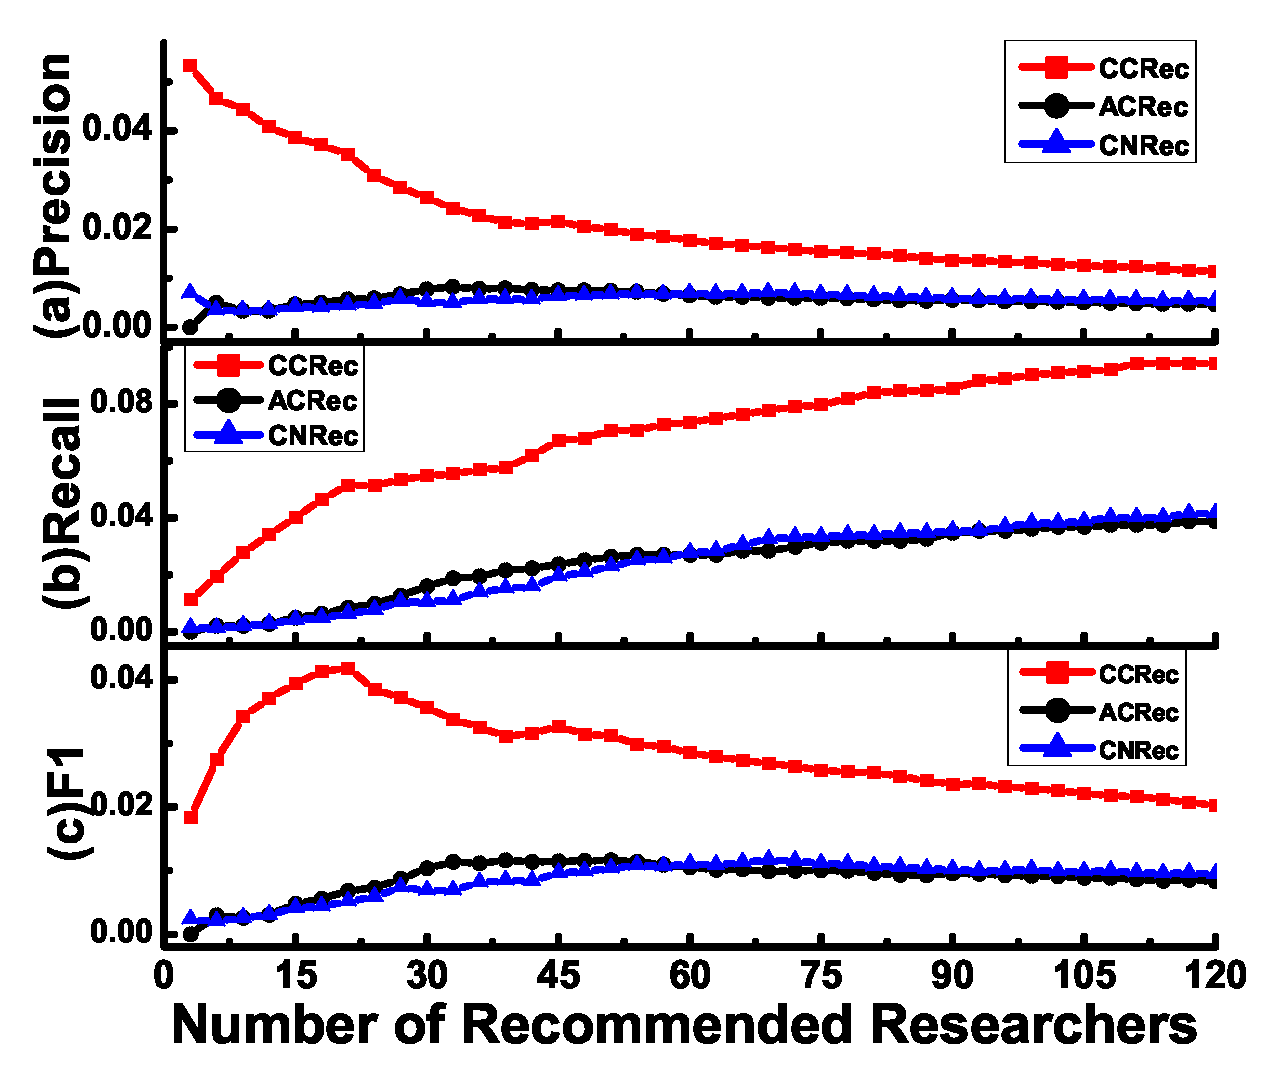
\includegraphics [width=3.4in]{Fig4.eps}
\caption{The impact of clustered domains number on CCRec}
\end{figure}

In terms of Fig. 4, the number of clustered domains does have certain effect on the performance of CCRec. If the number of clustered domains is appropriate, the $F1$ score can get some enhancement. In this situation, when clustering the data mining academia into 300 or 500 domains, CCRec performs best for $F1$, which reaches $4.18\%$.

In summary, we can still claim that the model combining content-based method and social networks-based method is really effective. Moreover, in terms of precision, recall and $F1$, CCRec outperforms ACRec and CNRec on making most potential collaborators recommendation for academic researchers.
% =============================================================================
\section{Conclusions}
% =============================================================================
In this paper, we focused on how to find researchers' MPCs based on big scholarly data which is necessary in current academia. To this end, we proposed a novel model named CCRec, by combining the features of publications content and collaboration networks. A topic clustering model and A random walk model are adopted to obtain the scholars features, and make MPCs recommendation for researchers. We conducted extensive experiments on a subset of DBLP data set to evaluate the performance of CCRec. We also conducted the ACRec and CNRec on the data set as comparisons. The experimental results show that, CCRec outperforms ACRec and CNRec in precision, recall and $F1$ score. With employing topic clustering model, the problem of topic drift has been solved to some extent.

Our research on CCRec reveals that the combination of content-based method and networks-based method can improve the generation of effective academic collaborations. Nonetheless, there is still room for future study in this direction. We extracted the titles of publications as the corpus of topic clustering model, which are not more comprehensive than the abstract and main body of publications. Besides, an exactly metric should be confirmed to evaluate the topic drift problem. As future work, more experiments and studies should be conducted.

\section*{References}

\bibliography{CCRec-Full}

\end{document}
